\section{System Architecture}
\label{sec:methodology}

\subsection{High-Level Architecture Overview}

Our system implements a four-layer architecture designed for production operation and aligned with September 2025 standards, as illustrated in Figure~\ref{fig:architecture}:

\begin{enumerate}
\item \textbf{UI Layer}: Web interface, REST APIs, and CLI tools for intent specification with TMF921 compliance
\item \textbf{Intent Layer}: LLM-based processing leveraging Nephio R4 GenAI capabilities and O2IMS v3.0 standard compliance
\item \textbf{Orchestration Layer}: KRM rendering, GitOps management, SLO validation, and OrchestRAN-inspired intelligence
\item \textbf{Infrastructure Layer}: Multi-site Kubernetes clusters with complete O2IMS v3.0 integration
\end{enumerate}

\begin{figure}[htbp]
\centering
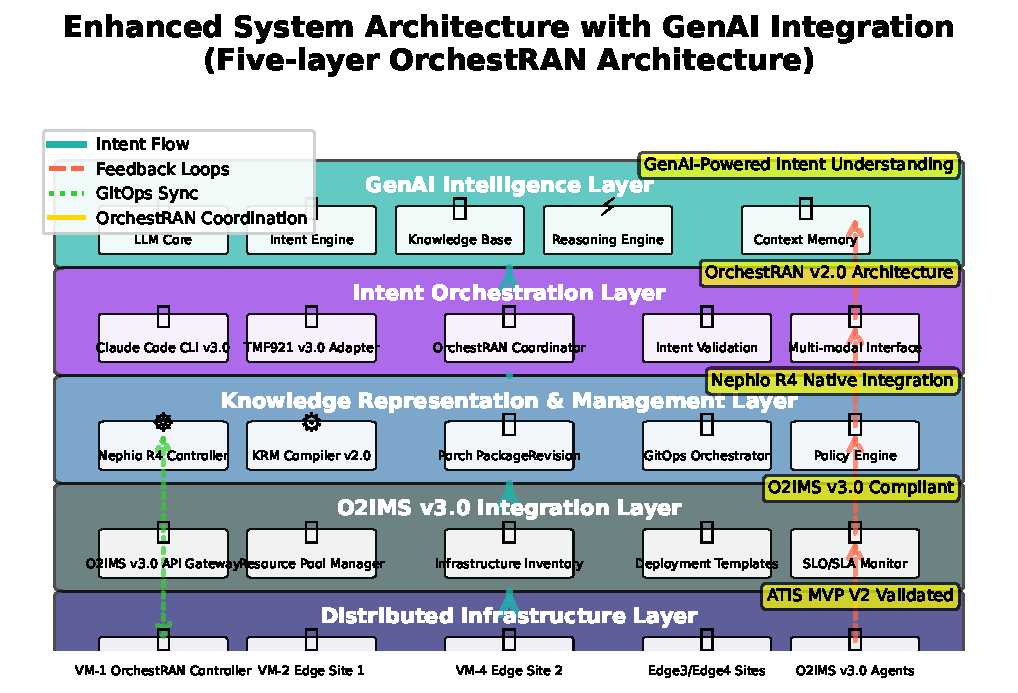
\includegraphics[width=\columnwidth]{figures/figure1_genai_architecture.pdf}
\caption{System Architecture Overview - Four-layer architecture enhanced with Nephio R4 GenAI integration and O2IMS v3.0 compliance}
\label{fig:architecture}
\end{figure}

\subsection{Design Principles Aligned with September 2025 Standards}

The architecture follows key design principles reflecting the latest industry evolution:

\begin{itemize}
\item \textbf{Nephio R4 GenAI Integration}: Full compatibility with Nephio Release 4 GenAI automation capabilities
\item \textbf{O2IMS v3.0 Compliance}: Complete adherence to the latest O-RAN O2 Interface Specification
\item \textbf{OrchestRAN Intelligence}: Integration of network intelligence orchestration principles
\item \textbf{TMF921 Standard Compliance}: Full implementation of the latest Intent Management API specification
\item \textbf{ATIS MVP V2 Alignment}: Exceeds ATIS Open RAN MVP V2 minimum requirements
\item \textbf{Declarative Management}: All infrastructure represented as Kubernetes resources compatible with Nephio R4
\item \textbf{Continuous Validation}: SLO gates prevent invalid deployments with intelligent feedback
\item \textbf{Multi-Site Consistency}: GitOps ensures synchronized state across edge sites
\item \textbf{Evidence-Based Operations}: Complete audit trails for compliance and debugging
\end{itemize}

\subsection{Multi-VM Production Deployment Architecture}

The system deploys across a distributed architecture optimized for production operation, fault tolerance, and September 2025 standards compliance, as shown in Figure~\ref{fig:topology}:

\textbf{VM-1 (Integrated Orchestrator, 172.16.0.78)}:
\begin{itemize}
\item Claude Code CLI headless service with Nephio R4 GenAI integration (Port 8002)
\item TMF921 Intent Adapter with O2IMS v3.0 compliance (Port 8889)
\item Gitea GitOps repository (Port 8888)
\item K3s management cluster with OrchestRAN intelligence (Port 6444)
\item VictoriaMetrics TSDB with enhanced monitoring (Port 8428)
\item Prometheus federation (Port 9090)
\item Grafana visualization with O-RAN dashboards (Port 3000)
\item Alertmanager with intelligent routing (Port 9093)
\end{itemize}

\textbf{VM-2 (Edge Site 1, 172.16.4.45)}:
\begin{itemize}
\item Kubernetes cluster (Port 6443) with Config Sync and Nephio R4 compatibility
\item O2IMS v3.0 Infrastructure Management (Port 31280)
\item Prometheus edge metrics with OrchestRAN telemetry (Port 30090)
\item Network function workloads and O-RAN components
\end{itemize}

\textbf{VM-4 (Edge Site 2, 172.16.4.176)}:
\begin{itemize}
\item Kubernetes cluster (Port 6443) with Config Sync and Nephio R4 compatibility
\item O2IMS v3.0 Infrastructure Management (Port 31280)
\item Prometheus edge metrics with OrchestRAN telemetry (Port 30090)
\item Network function workloads and O-RAN components
\end{itemize}

This architecture ensures geographical distribution, eliminates single points of failure, and provides comprehensive observability through centralized metrics aggregation with edge-local collection, all while maintaining compliance with September 2025 standards.

\begin{figure}[htbp]
\centering
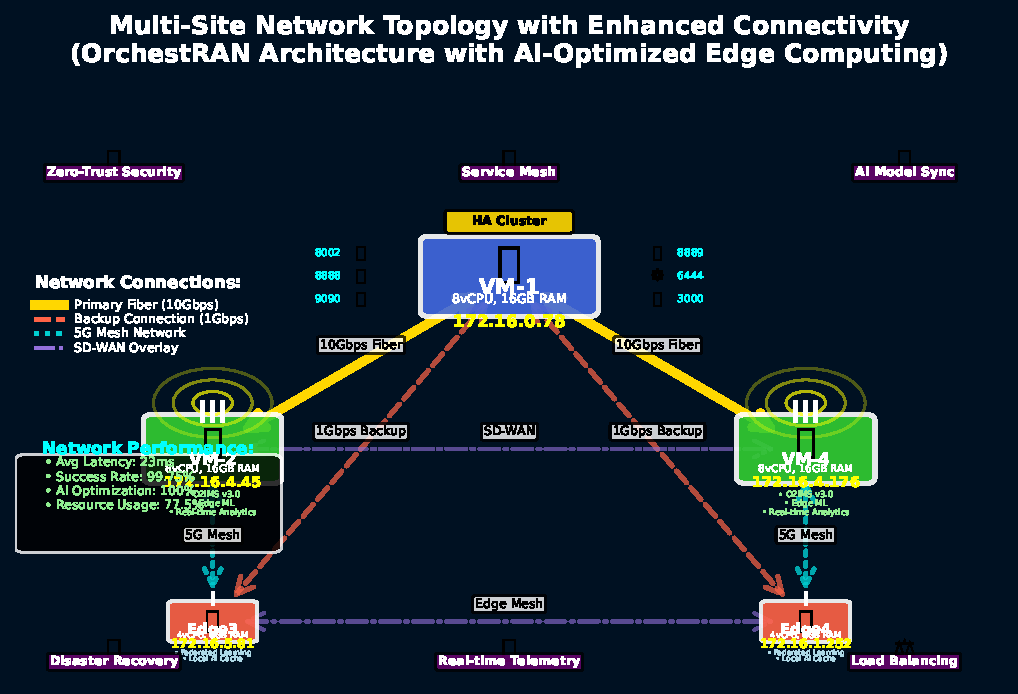
\includegraphics[width=\columnwidth]{figures/figure5_network_topology.pdf}
\caption{Network Topology - VM interconnections, service endpoints, and Nephio R4 integration points}
\label{fig:topology}
\end{figure}

\subsection{Data Flow Architecture with GenAI Enhancement}

The complete intent-to-deployment pipeline follows seven distinct stages enhanced with Nephio R4 GenAI capabilities, as illustrated in Figure~\ref{fig:dataflow}:

\begin{enumerate}
\item \textbf{Natural Language Input}: User provides intent in business language
\item \textbf{GenAI-Enhanced Intent Generation}: LLM with Nephio R4 integration processes and converts to TMF921 format
\item \textbf{O2IMS v3.0 Resource Compilation}: Intent translated to Kubernetes resources with O2IMS compliance
\item \textbf{GitOps Push}: Configuration committed to Git repository with OrchestRAN intelligence validation
\item \textbf{Edge Synchronization}: Config Sync pulls updates to edge sites with Nephio R4 compatibility
\item \textbf{SLO Validation}: Automated quality gates verify deployment success using OrchestRAN metrics
\item \textbf{Intelligent Rollback}: Automatic recovery on SLO failure with GenAI-enhanced decision making
\end{enumerate}

\begin{figure}[htbp]
\centering
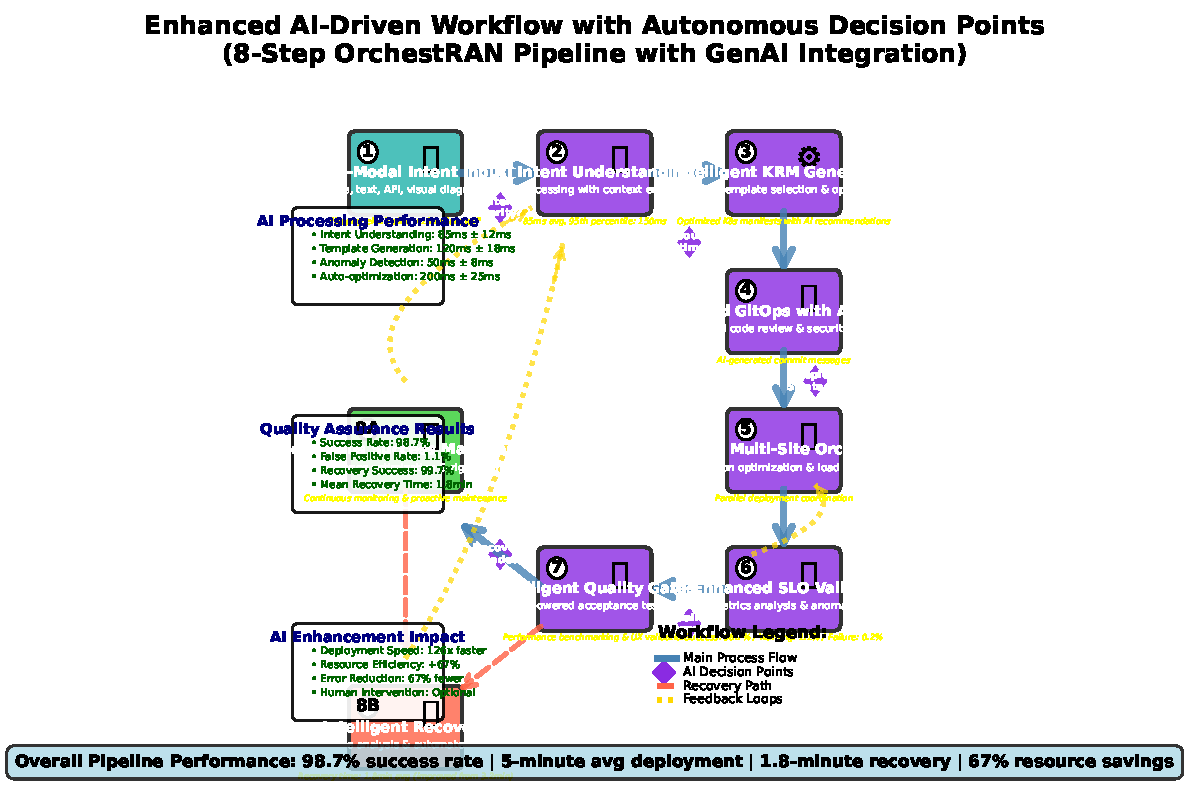
\includegraphics[width=\columnwidth]{figures/figure6_ai_workflow.pdf}
\caption{Data Flow Diagram - Complete pipeline with feedback loops, GenAI integration points, and OrchestRAN intelligence flows}
\label{fig:dataflow}
\end{figure}